\chapter{Visualization for Explainable Classifiers}\label{sec-visualization}

As discussed at the end of \autoref{sec-explainable-classifier}, current research only focuses on one subject of the problem of explainable classifier and neglects the other subject -- human. Thus, we study explainable classifier from the aspects of visualization and human computer interaction in this chapter. Broadly speaking, the visualization for explainable classifiers can be viewed as a special case of algorithm visualization or software visualization. The former aims to provide better understanding of algorithms for education purposes in computer science. The latter focus on assisting developers and operation engineers for the development and maintenance of complex software. Here, the subject of visualization is the classifiers, which can be treated as algorithms learned from the data, or complex systems that need assistance in understanding.
% Unlike the previous chapter that discuss various algorithms for enhancing the explaianbility of classifiers,

We view the development and the operation of an intelligent system as a system engineering problem, and divide the life cycle of an intelligent system into different stages. The classification system can be treat as a specification of the general intelligent system. Then, we identify the current issues in explaining classifiers and discuss the research opportunities of visualization regarding different stages.

\section{Life Cycle of an intelligent system}

\begin{figure}[hb]
    \centering
    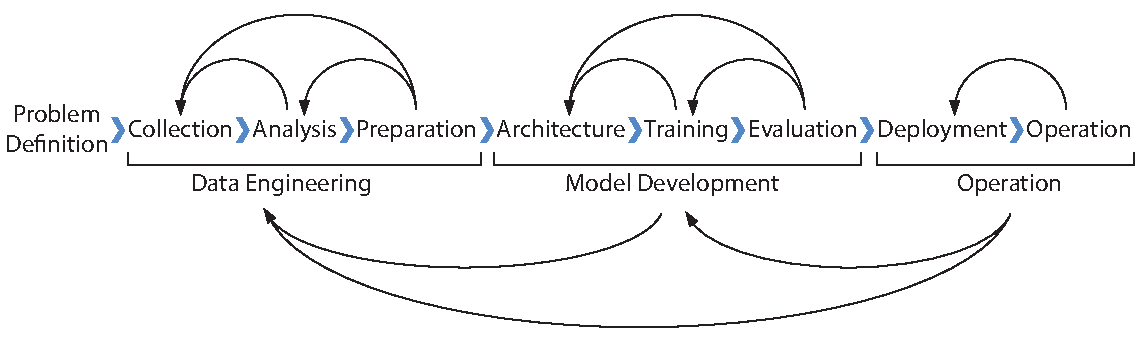
\includegraphics[width=1.0\textwidth]{figure/life-cycle}
    \caption{The life cycle of a classifier.}
    \label{fig:life-cycle}
\end{figure}

A classification system can be thought as a specialized case af an intelligence system. An intelligent system is developed to perform certain tasks with artificial intelligence (here we only consider data-driven systems). 
The development of a data-driven intelligent system is an iterative process. In this survey, the entire life cycle of an intelligent system is divided into three major stages (data engineering, model development, and operation) and eight sub-procedures (see \autoref{fig:life-cycle}). This definition is formed based on the cross-industry standard process for data mining \cite{wirth2000crisp}, a professional advice from Gartner, Inc. \cite{carlton2017ml}, the life cycle for expert system \cite{lasalle1990expert-system}, and the machine learning workflow of Google Cloud\footnote{\url{https://cloud.google.com/ml-engine/docs/ml-solutions-overview}}.

The first stage, data engineering, is defined to include any procedures that are data-related, namely, data collection, exploratory analysis, data preparation. The second stage, model development, includes procedures such as designing the architecture of the classifier (\eg, what type of model to use and parameters), training the model using data prepared, and evaluating whether the model meets certain requirements. After developing a classifier, the model is deployed, and in certain cases, is operated by some people. As we can see from \autoref{fig:life-cycle}, there are back-links from each stage/step to its previous stages/steps. This is the nature development. For example, we have a model with unsatisfactory performance after the training. This might due to model used is not suitable for certain tasks (go back to architecture setting), or it is because the volume of the data is too small (go back to collect more data). Similar problems might occur in other stages or procedures, which force us to go back and improve. 
%For example, if we are to develop a system for hospitals to detect early signs of lung cancer from a CT scan, the procedure goes as: 

Visualization and visual analytics systems are semi-automatic solutions at different stages to make a classifier more explainable. At the stage of data engineering, data visualization can help humans explore the data and get a qualitative sense of the nature of the data. Since the training of a classifier is actually extracting information from the training data, with more knowledge of the data in mind, humans (\ie developers or data scientists) can better understand if a failure results from the quality or volume issues of the data. At the second stage, visual analytics systems serve as development tools, which make the development more transparent and understandable. When designing or selecting model architectures, visual analytics systems can help humans better understand the characteristics of different classifiers, and even inspire improvements in the architecture. Visual diagnosing tools can help identify the problems in the training process and improve the debugging efficiency. For evaluations, visual analytics systems can help compare different classifiers and qualitatively evaluate the robustness and fairness of a classifier. At the last stage, when a classification system is deployed, visualization can help explain the inner workings of the system to end-users. For routine operations, visualization can better explain the predictions of the system, which make the monitoring and management easier. Also note that, visualization can used in the life-cycle for other purposes instead of explainability. For example, monitoring the training process by plotting loss curves, or visualization for crowd sourcing to collect data with better quality.

-------

A table summarizing all related papers

-------

\section{Visualization for Data Understanding}

At the stage of data engineering, visualization can be used mainly in the procedure of data analysis to assist humans' understanding of the data. Data plays an important role in the success of machine learning advances. A trained classifier can be viewed as a machine that has extracted the information in the training data and abstracted the information as its parameters. Thus, understand the data is the first step to understand a classifier.

There is a long history of research in visualization for exploratory data analysis. When comes to the 


\section{Visualization for Model Development}

There is a surge of interest to use visualization for explainable classifiers, focusing on the stage of model development. We summarized three tasks for visualization, namely, model understanding, model diagnosing, and assessment and comparison, which are corresponding to the three stages: architecture design, training, and evaluation.

\subsection{Understanding}

Scientific understanding. Investigate the characteristic of the model.

Existing work:

\subsection{Diagnosing}

Diagnose model and data.

Existing work: 

\subsection{Assessment and Comparison}

Unquantifiable assessments, Fairness (e.g., discrimination), Vulnerability

Existing work: 

\section{Visualization for Model Operation}
\subsection{Trust Establishment}
\subsection{Monitoring}

\section{Other Applications}
\subsection{Teaching and Communicating Models}
Narrative, Interactive, etc. to explain your model to others.
\subsection{Learn from the Model} 
Knowledge Discovery; Learn lessons from what the model learned (Alpha Go)

\section{Evaluation}

Review methods and standards of evaluating visualization.

Address the problem of the lack of evaluation standards for visualization for explaianble classifiers.

Proposed?

1. Fidelity. How visualization reflects the real model. (The relativeness and faithfulness of explanation)

2. Understandability. How easy the visualization is to be understood.

\newpage

